\documentclass{article}
\usepackage[utf8]{inputenc}
\usepackage{graphicx}
\graphicspath{ {./} }

% \title{EulerAlgoGCD}
% \author{Glaives De Vérité}
% \date{December 2022}
\begin{document}
\begin{flushleft}
\textbf{Algorithm E} (\textit{Euclid's Algorithm}). Given two positive integers \textit{m} and \textit{n}, find their \textit{greatest common divisor}, that is, the largest positive integer that evenly both \textit{m} and \textit{n}.
\vspace{4mm}
\par \textbf{E0.} [Ensure $\textit{m}\geq\textit{n}$.] If $\textit{m}<\textit{n}$, exchange $\textit{m}\Leftrightarrow\textit{n}$.
\vspace{2mm}
\par \textbf{E1.} [Find  remainder.] Divide \textit{m} by \textit{n} and let \textit{r} be the remainder. (We will have $0\leq\textit{r}<\textit{n}$.)
\vspace{2mm}
\par \textbf{E2.} [Is it zero?] If $\textit{r}=0$, the algorithm terminates; \textit{n} is the answer.
\vspace{2mm}
\par \textbf{E3.} [Reduce.] Set $\textit{m}\gets\textit{n}$, $\textit{n}\gets\textit{r}$, and go back to step \textbf{E1}.
\vspace{3mm}
\par 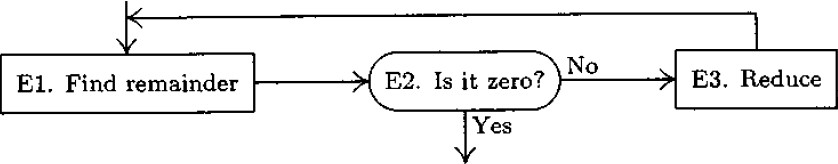
\includegraphics[width=\textwidth]{scheme}
\end{flushleft}

\end{document}

% \maketitle

